\documentclass{beamer}
\usetheme{metropolis}    
\usepackage{amsmath}
\usepackage{textcomp}
\usepackage{stmaryrd}
\usepackage{tikz} 
%Information to be included in the title page:
\title{What is algebraic about algebraic effects and handlers?}
\author{Łukasz Magnuszewski}
%\institute{Overleaf}
\date{2023}

\begin{document}

\frame{\titlepage}

\begin{frame}
\frametitle{Outline}
\tableofcontents[sections=1-2]
\end{frame}
\begin{frame}
    \frametitle{Outline}
    \tableofcontents[sections=3-5]
    \end{frame}
    

\section{Algebraic theories}

\begin{frame}
\frametitle{Algebraic theories}

\begin{example}
    Group is a structure $(G, u, *, ^{-1})$ satisfying following equations:

   \[
    (x * y) * z = x * (y * z) 
   \]
   \[
    (u * x) = x = x * u 
   \]
   \[
    x * x^{-1} = u = x^{-1} * x
   \]
        
    
\end{example}
We can define group using other definitions (using quantifiers), 
but we will stick to this type of definitions, known as algebraic or equational theories.

\end{frame}

\subsection{Signatures}

\begin{frame}{Signatures}
    \begin{definition}
        Signature $\Sigma$ is a collection of \textit{operation symbols} with \textit{arities}
        $\{(op_i, ar_i)\}_i$
       
        
        The operation symbols $op_i$ can by anything, 
          but we usually think about them as syntactic entities
        
        
        The arities $ar_i$ are non-negative-integers


        
    \end{definition}
    
    Operation symbols with 0 arity is constant, while operation symbol with 1, 2, 3 arities are
    unary, binary, ternary, respectively. 

    
    \begin{example}
        Signature for group is 
        \[
          \{ u, 0 \}, \quad \{ ^{-1}, 1 \}, \quad \{ *, 2 \} 
        \]
    \end{example}

\end{frame}

\subsection{Terms}
\begin{frame}
    \frametitle{Terms}
    \begin{definition}
        Context is (possibly empty) list of distinct variable $x_1, \ldots, x_k$
    \end{definition}

    \begin{definition}
        $\Sigma$-terms in context $x_1, \ldots, x_k$ are build inductively from following rules
        \begin{itemize}
            \item variable $x_i$ is as $\Sigma$-term in context $x_1, \ldots, x_k$
            \item if $t_1, \ldots, t_{ar_i}$ are $\Sigma$-terms in context $x_1, \ldots, x_k$ 
            then $op_i(t_1, \ldots, t_{ar_i})$ is a $\Sigma$-term in context $x_1, \ldots, x_k$
        \end{itemize}
       

    \end{definition}

    \begin{example}
        Using signature of group
        following terms
        \[
          a * (b * c),\quad a^{-1} * a,\quad u,\quad u * c  
        \] are $\Sigma$-terms in context a, b, c
    \end{example}
\end{frame}


\subsection{Equations}
\begin{frame}
    \frametitle{$\Sigma$-Equations}
    \begin{definition}
        $\Sigma$-equation is a pair of $\Sigma$-terms l and r in a context $x_1, \ldots, x_k$. We write
        \[
            x_1, \ldots, x_k | l = r   
        \]
    \end{definition}
    \begin{example}
        $\Sigma$-equations for group:
        \begin{enumerate}
            \item $x, y, z | (x * y) * z = x * (y * z)$
            \item $x | x * u = x$
            \item $x | u * x = x$
            \item $x | x * x^{-1} = u$
            \item $x | x^{-1} * x = u$
        \end{enumerate}
    \end{example}


\end{frame}

\subsection{Algebraic theories}
\begin{frame}
    \frametitle{Algebraic theory}
    \begin{definition}
        Algebraic theory $T = (\Sigma_T, \mathcal{E}_T)$ is given by a signature
        $\Sigma_T$ and a collection $\mathcal{E}_T$ of $\Sigma_T$-equations.
    \end{definition}
    \begin{example}{Theory of groups:}
        

        $\Sigma_T = \{ u, 0 \}, \quad \{ ^{-1}, 1 \}, \quad \{ *, 2 \} $

        $\mathcal{E}_T$:
        \begin{enumerate}
            \item $x, y, z \quad |\quad (x * y) * z = x * (y * z)$
            \item $x \quad | \quad x * u = x$
            \item $x \quad |\quad u * x = x$
            \item $x \quad| \quad x * x^{-1} = u$
            \item $x \quad | \quad x^{-1} * x = u$
        \end{enumerate}
    \end{example}

\end{frame}
\begin{frame}
    \frametitle{Simple examples of algebraic theories}

    \begin{example}
        Theory of pointed set has a constant $\circ$ and no equations
    \end{example}


    \begin{example}
        Empty theory has no operations symbols and no equations 
    \end{example}


    \begin{example}
        Theory of singleton has a constant $\circ$ and the equation $x = y$.
    \end{example}

\end{frame}

\section{Interpretations and Models}

\subsection{Interpretations of signatures}

\begin{frame}
    \frametitle{Interpretations of signatures}
    \begin{definition}
        An Interpretation $I$ of signature $\Sigma$ is given by
        \begin{enumerate}
            \item a set $|I|$, called the carrier
            \item for each operation symbol $op_i$ a map
                \[
                    \llbracket op_i \rrbracket_I : \underbrace{|I| \times \ldots \times |I|}_{ar_i} \rightarrow  |I|
                \]
            called an operation
        \end{enumerate}
    \end{definition}

\end{frame}

\begin{frame}
    \frametitle{Interpretations of $\Sigma$-terms}
    \begin{definition}
        An Interpretation of $\Sigma$-term in context is interpreted by a map
        \[
          \llbracket x_1, \ldots , x_k  | t \rrbracket_I : |I|^k -> |I|
        \]
  The variable $x_i$ is interpreted as the $i$-th projection
            \[
                \llbracket x_1, \ldots , x_k  | x_i \rrbracket_I = \pi_i : |I|^k \rightarrow |I|
            \]

A compund term 
                \[
                    x_1, \ldots , x_k \quad  | \quad op_i(t_1, \ldots , t_{ar_i}  )
                \]
                is interpreted as the composition of maps 
                \[
                    |I|^k \xrightarrow{(\llbracket t_1\rrbracket_I, 
                    \ldots {\llbracket t_{ar_i}\rrbracket_I}) } |I|^{ar_i} \xrightarrow{
                        \llbracket op_i \rrbracket_I} |I|
                \]



    \end{definition}
\end{frame}

\subsection{Models of theories}
\begin{frame}
    \frametitle{Model of algebraic theories}
    \begin{definition}
        Model $|M|$ of an algebraic theory $T$ is an interpretation of the signature $\Sigma_T$
        which validates all the equations $\mathcal{E}_T$. That is for every equation
        \[
          x_1, \ldots, x_k | l = r   
        \]
        in $\mathcal{E}_T$, the maps 
        \[
          \llbracket x_1, \ldots, x_k | l \rrbracket_M  
           \quad and \quad \llbracket x_1, \ldots, x_k | r \rrbracket_M  
        \]
        are equal.
    \end{definition}

    

\end{frame}

\begin{frame}
    \frametitle{Homomorphisms of models}
    \begin{definition}
        Suppose L and M are models of a theory T. A T-homomorphism from L to M is a map
        $\phi : |L| \rightarrow |M |$
        which commutes with operations: for every operation symbol $op_i$ of T, we have
        \[
            \phi \circ \llbracket op_i \rrbracket_L = \circ \llbracket op_i \rrbracket_M \circ 
            \underbrace{\phi, \ldots, \phi}_{ar_i}
        \]
    \end{definition}    

\end{frame}

\subsection{Free Models}
\begin{frame}
    \frametitle{Free Models}
    \begin{definition}
        Given an
        algebraic theory T and a set X, the free T-model, also called the free T-algebra, generated
        by X is a model M together with a map $\eta : X \rightarrow |M|$ such that, for every T-model L and
        every map $f : X \rightarrow |L|$ there is a unique T-homomorphism $\overline{f} : M \rightarrow L$ for which the
        following diagram commutes:
    
    
        \begin{center}
            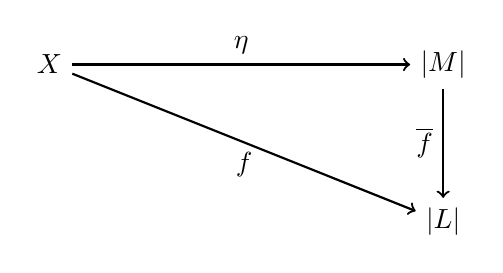
\begin{tikzpicture}[thick]
            \path 
            (0,0)       node (X) {$X$}
            +(5,0)  node (M) {$|M|$}
            +(5, -2) node (L) {$|L|$};
            \draw[->] (X)--(M) node[pos=.5,above]{$\eta$};
            \draw[->] (X)--(L) node[pos=.5,below]{$f$};
            \draw[->] (M)--(L) node[pos=.5,left]{$\overline{f}$};
            \end{tikzpicture}
            \end{center}    
    
            We can understand this that free T-model generated by x is the "most economical"
            way of making a T-model out of the set X.
    \end{definition}
\end{frame}

\begin{frame}
    \frametitle{Every algebraic theory have free model}
    First we take set of all well founded trees with operation symbols from $T_\Sigma$ and variables 
    from X. Let that be $Tree_\Sigma(X)$ defined as follows 
    \begin{enumerate}
        \item for each $x \in X$, there a tree $return x \in Tree_\Sigma(X)$
        \item for each $op_i$ and trees $t_1, \ldots, t_{ar_i}$ theere is a tree denoted by 
        $op_i(t_1, \ldots, t_{ar_i}) \in Tree_\Sigma(X)$, whose root is labeled by $op_i$ and whose
        subtrees are $t_1, \ldots, t_{ar_i}$
    \end{enumerate}
    The $\Sigma$-terms in context $x_1, \ldots, x_n$ are precisely the trees in $Tree_\Sigma(\{x_1, \ldots, x_n\})$
    except that a variable $x_i$ is labeled as return $x_i$ when construed as a tree
\end{frame}

\begin{frame}
    \frametitle{Every algebraic theory have free model}
    Given a theory T, let $\approx_T$ be the least congruence relation 
    such that every equation is satisfied.
    Define the carrier of the free mode $F_T(X)$ to be the quotient set
    \[
      |F_T(X) =   Tree_\Sigma(X)/\approx_T
    \] the interpretation of symbols is them map $\llbracket op_i \rrbracket_{F_T(X)}$ defined by
    \[
        \llbracket op_i \rrbracket_{F_T(X)}(|t_1|, \ldots, |t_{arr_i}|) =
        |op_i(t_1, \ldots, t_{arr_i})|   
    \]
    The map $\eta_X : X  \rightarrow  F_T(X)$ is defined by $\eta_X(x) = |return \, x|$.

    It can be verified that such construction is free model.
\end{frame}


    \subsection{Operations with general arities and parameters}
    \begin{frame}
        \frametitle{General arities}
        One idea to make general arities would be to write 
    \[
      op_i(\ldots, t_\alpha, \ldots)_{\alpha \in A}  
    \]
    But we know that 
    \[
      \underbrace{X \times  \ldots \times X}_{|A|} \cong X^A 
    \]
    And we can use $\lambda$-calculus to write such function.
    To have A-many elements of a set X is to have a map $\kappa : A -> X$.
    And to apply the operation symbol $op_i$ to a-many arguments $\kappa$ we simply write $op_i(\kappa)$.

    \end{frame}

    \begin{frame}
        \frametitle{Operations with parameters}
        To motivate parameters, consider theory of vector space $M$.

        We need to consider how to define multiplying vectors with scalars from $\mathbb{R}$
       There are 2 possibilities:
       \begin{enumerate}
        \item Instead of having a single binary operation taking a scalar and a vector, we could
        have many unary operations taking a vector, one for each scalar.
        \item We could view the scalar as an additional parameter of a unary operation on vectors
       \end{enumerate} 
       We shall adopt the second approach. We can generalize terms, equations, interpretations, 
       models, homomorphisms to work with arbitrary arity and parameters. 
    \end{frame}

    \begin{frame}
        \frametitle{Theory of vectors over $\mathbb{R}$}
        Lets define operations of this theory.

        Scalar multiplication is unary operation mul parametrized by elements of $\mathbb{R}$.
        That is fo over $r \in \mathbb{R}$ and term t we may write the term
        \[
          mul(r; t)  
        \]
        Other operation doesn't  need parameters, buw we can force them to take unit parameter
        for example addition of vectors 
        \[
          add((); t_1, t_2)  
        \]
    
        
    
    \end{frame}

 










    






\section{Computation effects as algebraic operations}

\begin{frame}
    \frametitle{Computation effects as algebraic operations}
    Its start to give some examples from programming. We can define many computations effects
    by algebraic theories.


    We can divide computations into two kinds (we are omitting non-terminating)
    \begin{enumerate}
        \item pure, which terminates and return value v, then we write 
        \[
          return \, v  
        \]
        \item effectful. Then we model this with operation which take parameter p, for instance the memory location to be read, or the string
        to be printed, and a continuation $\kappa$, which is a suspended computation expecting the result
        of the operation, for instance the contents of the memory location that has been read.
        \[
          op(p, \kappa)  
        \]
    \end{enumerate}
    
    
    \end{frame}

    \begin{frame}
        \frametitle{Algebraic theory of state}
        The algebraic theory of state with locations L and states S has operations
        \[
          lookup \, : \, L  \rightsquigarrow S \quad and \quad update \, : \, L \times S  \rightsquigarrow 1
        \]
        Take look at example computation l++
        \[
            lookup(l, \lambda \, x. update((l, x + 1), \lambda \textunderscore. return x))
        \]
      
    
    \end{frame}
    
    \begin{frame}
        \frametitle{Equations for successive lookups and updates}
        First we have equations which state what happens on successive lookups and updates to
        the same memory location. For all $l \in L$, $s \in S$ and all continuations $\kappa$
        \[
            lookup(l, \lambda s . lookup(l, \lambda t . \kappa s t)) = 
            lookup(l, \lambda s . \kappa s s)
        \]
        \[
            lookup(l, \lambda s . update((l, s), \kappa)) = \kappa ()
        \]
        \[
            update((l, s), \lambda \textunderscore . lookup(l, \kappa)) = update((l,s), 
            \lambda \textunderscore . \kappa s
            )
        \]
        \[
            update((l, s), \lambda \textunderscore . update((l,t), \kappa 
            )) =   update((l,t), \kappa 
            )
        \]
        
    
    \end{frame}

    \begin{frame}
        \frametitle{Lookups and updates from diffrent locations}
        There is a second set of equations stating that lookups and updates from different 
        locations $l  \neq l'$ distribute over each other:

        \[
            lookup(l, \lambda s. lookup (l',  \lambda s'. k \, s\, s'))
            = lookup(l', \lambda s'. lookup (l,  \lambda s. k \, s\, s'))
        \]
        \[
          update((l,s), \lambda \textunderscore. lookup(l', \kappa))  
          = lookup(l', \lambda t. update((l,s), \lambda \textunderscore. \kappa \, t))
        \]
        \[
            update((l,s), \lambda \textunderscore. update((l', s'), 
            \kappa))
            =   update((l',s'), \lambda \textunderscore. update((l, s), 
            \kappa))
        \]
    
        
    
    \end{frame}


    \begin{frame}
        \frametitle{Combining algebraic theories}
        Algebraic theories may be combined. For example, we want to combine state and I/O.
Sometimes we want to combine theories so that the operations between them interact.
To demonstrate this, let us consider the theory of a single stateful memory location holding
elements of a set S. The operations are
\[
  get : 1 \rightsquigarrow S \quad put : S \rightsquigarrow 1  
\]
    
        
    
    \end{frame}
    \begin{frame}
        \frametitle{Single State theory equations}
        The equations are:
        \[
            get((), \lambda s . get((), \lambda t . \kappa \, s \, t)) = 
            get((), \lambda s . \kappa \, s  \, s)
        \]
        \[
            get((), \lambda s . put(s, \kappa)) = \kappa ()
        \]
        \[
            put(s, \lambda \textunderscore . get((), \kappa)) = put(s, 
            \lambda \textunderscore . \kappa s
            )
        \]
        \[
            put( s, \lambda \textunderscore . put(t, \kappa 
            )) =   update(t, \kappa 
            )
        \]
        This is just the first group of equations from previous example, except that we need not specify
which memory location to read from.

    \end{frame}

    \begin{frame}
        \frametitle{Combining multiply states}
        That is, to model I-many states,
        we combine I-many copies of the theory of a single state, so that for every $l \in$ I we have
        operations
        \[
          get_l : 1 \rightsquigarrow S_l \quad and \quad   get_l : S_l \rightsquigarrow 1
        \]
        We also need to define how diffrent operations combine,
        \[
            get_l((), \lambda s. get_{l'} ((),  \lambda s'. k \, s\, s'))
            = get_{l'}((), \lambda s'. get_; ((),  \lambda s. k \, s\, s'))
        \]
        \[
          put_l(s, \lambda \textunderscore. get_{l'}((), \kappa))  
          = lookup_{l'}((), \lambda t. put_l(s, \lambda \textunderscore. \kappa \, t))
        \]
        \[
            put_l(s, \lambda \textunderscore. put_{l'}((), s'), 
            \kappa)
            =   put_{l'}(s', \lambda t. put_{l}((), \lambda \textunderscore., 
            \kappa))
        \]
        This theory is almost the same as theory of multiply locations with two differences, 
        we can have different states in each location. And instead giving parameter to operation, we index our operations.
    
    \end{frame}



    \subsection{Computation are free models}
    \begin{frame}
        \frametitle{Computation are free models}
        Consider the theory State from previous slides. Let us see that free model $F_{State}(V)$
        adequately describes stateful computations returning values from V.
        Every tree from $Tree_{\Sigma_{State}}(V)$ is congruent to one of the form 
        \[
          get((), \lambda s. put(f(s), \lambda \textunderscore. return g(s)))
        \]
        for some maps $f : S \rightarrow S$ and $g : S \rightarrow V$.
         Indeed, by applying the equations,
        we may contract any two consecutive gets to a single one, and similarly for
        consecutive puts, we may disregard a get after a put,
         and cancel a get followed by a put. And give constant continuation.

        Therefore the free model $F_{State}(V)$ is isomorphic to the set of functions $S \rightarrow S \times V$.
        
    
    \end{frame}
    \subsection{Sequencing and generic operations}
\begin{frame}
    \frametitle{Generic operations}

    Consider some syntactic sugar for our notation, the same which was presented three weeks ago.
    Consider an algebraic theory T. For an operation $op : P \rightsquigarrow A$ in $\Sigma_T$, define the
corresponding generic operation
\[
  \overline{op}(p) \, := \, op(p, \lambda x. return \, x)   
\]
In words, the generic version performs the operation and returns its result. When the
parameter is the unit we write $op()$ instead of the silly looking $op(())$. 
    

\end{frame}
\begin{frame}
    \frametitle{Sequencing operations}

    Suppose that 
    $t \in F_T(X)$ and $h : X \rightarrow F_T(X)$. We define syntactic sugar for sequencing. 
    first define helper function. 
    \[
        \phi^\dagger([return \, x]) = \phi(x),
    \] \[
        \phi^\dagger([op(p, \kappa)]) = [op(p, \phi^\dagger \circ \kappa)]
    \]
        The we can define do notation
    \[
      do \, x \leftarrow t \, in \, h(x) \, := \, h^\dagger(t)
      \]



\end{frame}


    
    
        

\section{Handlers}

\begin{frame}
    \frametitle{Handlers}
    So far the main take-away is that computations returning values from V and performing
operations of a theory T are the elements of the free model $F_T(V)$. What about transformations between computations, what are they?
    
We can define them as T-homomorphism between models 
\[
  H : F_T(V) \rightarrow |F_{T'}(V')|
\]


    

\end{frame}
\begin{frame}
    \frametitle{Handlers}
    So we need to give 3 things 
\begin{enumerate}
    \item a map $f \, : \, V \rightarrow |F_{T'}(V')|$
    \item for every $op_i \, : P_i \rightsquigarrow A_i \in \Sigma_T$, a map 
    \[
        h_i \, : \, P_i \times |F_{T'}(V')|^{A_i} \rightarrow |F_{T'}(V')|
    \]
    such that
    \item  the maps $h_i$ form a T-model on $|F_{T'}(V')|$ meaning the validate the equation of T.
\end{enumerate}
The map $H : F_T(V) \rightarrow |F_{T'}(V')|$ induced by that is the unique one satisfying 
\[
  H([return x]) = f(x) \quad and \quad H([op(p,\kappa)]) = h_i(p, H \circ \kappa)  
\]

\end{frame}

\begin{frame}
    \frametitle{Handlers notation}
    We need better notation for handlers. Let us write 
    \[
      handler \{  
        return \, x \, \mapsto \, f(x), \, (op_i(y; \kappa))_{op_i \in \Sigma_i}
      \}  
    \]
    For handler induced by $f$ and $h_i$, and 
    \[
      (with \, H \, handle \, C)  
    \] for the application of H to computation C.
    The defining equations for handlers written
in the new notation are:
\[
    (with \, H \, handle \, return \,  v \,) = f(v)  
\]
\[
  (with \, H \, handle \, do\,  x \, \leftarrow \, \overline{op_i}(p) \, in \, \kappa(x) )
  = h_i (p, \lambda x. \, with \, H \, handle \, \kappa(x))  
\]



    

\end{frame}

\section{What is coalgebraic about algebraic effects and handlers}

\begin{frame}
    \frametitle{Models of algebraic theories in a category}
    An interpretation I of theory T in category \textbf{C}(cartesian closed) is given by
    \begin{enumerate}
        \item an object $|I|$ in \textbf{C}, called the carrier,
        \item for each operation symbol $op_i$, a morphism in \textbf{C}
        \[
          \llbracket op_i \rrbracket_I : |I|^{ar_i} \rightarrow |I|  
        \]
    \end{enumerate}

        An interpretation is extended to $\Sigma$-terms in contexts as follows:
        $x_i$ is interpreted as i-th projection
        \[
          \llbracket x_1, \ldots x_k | x_i \rrbracket_I = \pi_i  
        \]
        Compound term $x_1, \ldots x_k | op_i(t_1, \ldots,t_{arr_i})$ is interpreted as the composition of morphisms:
        \[
            |I|^k \xrightarrow{(\llbracket t_1 \rrbracket_I), \ldots, (\llbracket t_{arr_i} \rrbracket_I)}
            |I|^{arr_i} \xrightarrow{ \llbracket op_i \rrbracket_I } |I|
        \]

    \end{frame}
\begin{frame}
    \frametitle{Comodels of theory}
    We will model top-level computation effects with comodels.
    A comodel of theory T in a category \textbf{C} is a model in the opposite category $\textbf{C}^{op}$.

    Recall that the interpretation of an operation $op_i \, : \, P \rightsquigarrow A$ in a model M is a map 
      $\rrbracket op \llbracket_M : P \times |M|^A \rightarrow |M|$
    which in the curried form is $|M|^A \rightarrow |M|^P$.
    In the opposite category the maps turns its direction, and the exponentials become products:
   
     \[ A \times |M| \leftarrow P \times |M| \]

     Thus, in a comodel W an operation $op : P \rightsquigarrow A$ is interpreted as map 
     \[
        \llbracket op \rrbracket^W :  P \times |W| \rightarrow A \times |W|
     \]
     which we call a cooperation
    

\end{frame}

\begin{frame}
    \frametitle{Examples of cooperations}

    \begin{example}
        Non-deterministic choice $choose : 1 \rightsquigarrow bool$ is interpreted as a cooperation:
        \[
          1 \times |W| \rightarrow bool \times |W|  
        \]
        If we think of $|W |$
as the set of all possible worlds, the cooperation choose is the action by which the world
produces a boolean value and the next state of the world.
    \end{example}

\begin{example}
    Exception $abort : 1 \rightsquigarrow \emptyset$ is interpreted as a cooperation:
    \[
      1 \times |W| \rightarrow  |W| \times \emptyset  
    \]
    Unless $|W|$ is the empty set, there is no such map. An exception cannot propagate to the
outer world. The universe is safe from segmentation fault
\end{example}
\end{frame}

\begin{frame}
    \frametitle{Examples of cooperations}
    \begin{example}
        Printing $print : S \rightsquigarrow 1$ is interpreted as a cooperation:
        \[
          S \times |W| \rightarrow  |W|  
        \]
        It is the action by which the world is modified according to the printed message 
    \end{example}
    \begin{example}
        Reading $read : 1 \rightsquigarrow S$ is interpreted as a cooperation:
        \[
          1 \times |W| \rightarrow  |W| \times S 
        \]
        This is quite similar to non-deterministic choice, except that the world provides an element
of S rather than a boolean value.
    \end{example}
 

    

\end{frame}
\begin{frame}
    \frametitle{Cointerpretations}
    A Cointerpretation of a signature $\Sigma_T$ is given by a carrier set $|I|$, and for each operation symbol
    $op : P \rightsquigarrow A$ a map 
    \[
      \rrbracket op \llbracket^I : P \times |I| \rightarrow A \times |I|  
    \]
    The cointerpretation I may be extended to well-founded trees as follows
    \begin{enumerate}
        \item the tree return x is interpreted as the x-th injection 
        \[
          \llbracket X \, | \, x \rrbracket^I : \omega \rightarrow (x, \omega) : |X| \times|I|   
        \]
        \item the tree $op_i(p, \kappa)$ is interpreted as 
         \[
            \llbracket X \, | \, op_i(p, \kappa) \rrbracket^I : |I| \rightarrow X \times |I|
        \]
        \[
            \llbracket X \, | \, op_i(p, \kappa) \rrbracket^I : \omega \rightarrow \llbracket X 
            | \kappa(a) \rrbracket^I (\overline{\omega}) 
            \quad where \, (a, \overline{\omega}) = \llbracket op_i \rrbracket^I(p, \omega)
        \]
       
    \end{enumerate}

    

\end{frame}
\begin{frame}
    \frametitle{Comodel}
    A comodel W of a theory T is a $\Sigma_T$-cointerpretation which validates all the equations $\mathcal{E}_T$.
As before, an equation is valid when the interpretations of its left- and right-hand sides
yield equal maps

    

\end{frame}
\begin{frame}
    \frametitle{Comodel of state}
    The operations of State are following $get : 1 \rightsquigarrow S$ and $put: S \rightsquigarrow 1$.
    so respective cooperations are $g: |W| \rightarrow S \times |W|$ and $p : S \times |W| \rightarrow |W|$.
    And cooperation must satisfy equations of State.
    Right and left side of equation $get((), \lambda s . put(s, \kappa)) = \kappa ()$  are 
    insterpreted as maps $|W| \rightarrow |W|$, namely 
    \[
      \llbracket \kappa () \rrbracket^W : w \mapsto w
    \]
    \[
      \llbracket get((, \lambda s). put(s, \kappa)) \rrbracket^W : w \mapsto p(g(w))   
    \]
    There are equal, precisely when, for all $w \in |W|, \quad p(g(w)) = w$.
    
 

\end{frame}
\begin{frame}
    \frametitle{Equations of comodel of state}
    We can treat similarly other equations which gives us that comodel of State must satisfy:
    \[
        p(g(w)) = w
    \]
    \[
      g(\pi_i(g(w))) = g(w)  
    \]
    \[
        g(p(s,w)) = (s, p(s,w))
    \]
    \[
      p(t, p(s,w)) = p(t, w)  
    \]

    

\end{frame}

\subsection{Tensoring comodels and models}

\begin{frame}
    \frametitle{Tensoring comodels and models}
    If we consider the elments of T-model $|M|$ as effectful computations and the element of $T$-comodel as 
    external environments it is natural to ask if combined together can be interpreted as running programs.
    
    Let $\sim_T$ be the least equivalence relation on $|M| \times |W|$
    such that, for every symbol $op : P \rightsquigarrow A$ in $\Sigma_T$, 
    and for all $p \in P, a \in A, \kappa : A \rightarrow |M|$. and $w, w' \in |W|$ 
    such that    \[
        \llbracket op \rrbracket^W    (p, w) = (a, w')
    \] then 
    \[
        (\llbracket op\rrbracket_M (p,\kappa), w)   \sim_T (\kappa(a), w')
    \]
    Define the tensor $M \otimes W$ to be the quotient set $(|M| \times |W|)/_{\sim_T}$
    
    
    

\end{frame}


\begin{frame}
    \frametitle{Tensor of state}
    Let us compute the tensor of $M = F_{State}(X)$, the free model of the theory of state generated by X, and the comodel 
    $W$  defined by 
    \[
      |W| := S, \quad \llbracket get \rrbracket^W := \lambda s. (s, s), \quad   \llbracket put \rrbracket^W := \lambda (s, t), s
    \]
    We may read the equivalences as rewrite rules, of executing programs, until we are left with $(\llbracket return \, x \, \rrbracket_M, s)$
    \[
      (\llbracket get((), \kappa)\rrbracket_M , s) \sim_{State} ( \llbracket \kappa \rrbracket_M (s), s)
    \]
    \[ 
        (\llbracket put(t, \kappa)\rrbracket_M , s) \sim_{State} ( \llbracket \kappa \rrbracket_M (), t)  
    \]

   Because $(\llbracket return \, x \, \rrbracket_M, s) \sim_{State} 
   (\llbracket return \, y \, \rrbracket_M, t)$ only if $x = y \, and \, s = t$ (proof ommited). 
   It follows that $M \otimes W \cong X \times S$.  In other words, the execution of a program in an initial
   state always leads to a return value paired with the final state

    

\end{frame}



\section{Homework}
\begin{frame}
    \frametitle{Homework}
    \begin{enumerate}
        \item Describe some computation effect with algebraic theory
        \item Describe free model of the theory T of an associative operation with a unit.
            It has constant $\epsilon$ and binary operation $*$ satisfying equations:
            \[
                (x * y) * z = x * (y * z)
            \]
            \[
                \epsilon * x = x
            \]
            \[
              x * \epsilon = x   
            \]
            Give a useful description of the free model of T generated by a set X. 
        
    \end{enumerate}
    
    

\end{frame}



\end{document}